% Options for packages loaded elsewhere
\PassOptionsToPackage{unicode}{hyperref}
\PassOptionsToPackage{hyphens}{url}
%
\documentclass[
]{book}
\usepackage{lmodern}
\usepackage{amssymb,amsmath}
\usepackage{ifxetex,ifluatex}
\ifnum 0\ifxetex 1\fi\ifluatex 1\fi=0 % if pdftex
  \usepackage[T1]{fontenc}
  \usepackage[utf8]{inputenc}
  \usepackage{textcomp} % provide euro and other symbols
\else % if luatex or xetex
  \usepackage{unicode-math}
  \defaultfontfeatures{Scale=MatchLowercase}
  \defaultfontfeatures[\rmfamily]{Ligatures=TeX,Scale=1}
\fi
% Use upquote if available, for straight quotes in verbatim environments
\IfFileExists{upquote.sty}{\usepackage{upquote}}{}
\IfFileExists{microtype.sty}{% use microtype if available
  \usepackage[]{microtype}
  \UseMicrotypeSet[protrusion]{basicmath} % disable protrusion for tt fonts
}{}
\makeatletter
\@ifundefined{KOMAClassName}{% if non-KOMA class
  \IfFileExists{parskip.sty}{%
    \usepackage{parskip}
  }{% else
    \setlength{\parindent}{0pt}
    \setlength{\parskip}{6pt plus 2pt minus 1pt}}
}{% if KOMA class
  \KOMAoptions{parskip=half}}
\makeatother
\usepackage{xcolor}
\IfFileExists{xurl.sty}{\usepackage{xurl}}{} % add URL line breaks if available
\IfFileExists{bookmark.sty}{\usepackage{bookmark}}{\usepackage{hyperref}}
\hypersetup{
  pdftitle={Quantifying Life},
  pdfauthor={Dmitry Kondrashov},
  hidelinks,
  pdfcreator={LaTeX via pandoc}}
\urlstyle{same} % disable monospaced font for URLs
\usepackage{color}
\usepackage{fancyvrb}
\newcommand{\VerbBar}{|}
\newcommand{\VERB}{\Verb[commandchars=\\\{\}]}
\DefineVerbatimEnvironment{Highlighting}{Verbatim}{commandchars=\\\{\}}
% Add ',fontsize=\small' for more characters per line
\usepackage{framed}
\definecolor{shadecolor}{RGB}{248,248,248}
\newenvironment{Shaded}{\begin{snugshade}}{\end{snugshade}}
\newcommand{\AlertTok}[1]{\textcolor[rgb]{0.94,0.16,0.16}{#1}}
\newcommand{\AnnotationTok}[1]{\textcolor[rgb]{0.56,0.35,0.01}{\textbf{\textit{#1}}}}
\newcommand{\AttributeTok}[1]{\textcolor[rgb]{0.77,0.63,0.00}{#1}}
\newcommand{\BaseNTok}[1]{\textcolor[rgb]{0.00,0.00,0.81}{#1}}
\newcommand{\BuiltInTok}[1]{#1}
\newcommand{\CharTok}[1]{\textcolor[rgb]{0.31,0.60,0.02}{#1}}
\newcommand{\CommentTok}[1]{\textcolor[rgb]{0.56,0.35,0.01}{\textit{#1}}}
\newcommand{\CommentVarTok}[1]{\textcolor[rgb]{0.56,0.35,0.01}{\textbf{\textit{#1}}}}
\newcommand{\ConstantTok}[1]{\textcolor[rgb]{0.00,0.00,0.00}{#1}}
\newcommand{\ControlFlowTok}[1]{\textcolor[rgb]{0.13,0.29,0.53}{\textbf{#1}}}
\newcommand{\DataTypeTok}[1]{\textcolor[rgb]{0.13,0.29,0.53}{#1}}
\newcommand{\DecValTok}[1]{\textcolor[rgb]{0.00,0.00,0.81}{#1}}
\newcommand{\DocumentationTok}[1]{\textcolor[rgb]{0.56,0.35,0.01}{\textbf{\textit{#1}}}}
\newcommand{\ErrorTok}[1]{\textcolor[rgb]{0.64,0.00,0.00}{\textbf{#1}}}
\newcommand{\ExtensionTok}[1]{#1}
\newcommand{\FloatTok}[1]{\textcolor[rgb]{0.00,0.00,0.81}{#1}}
\newcommand{\FunctionTok}[1]{\textcolor[rgb]{0.00,0.00,0.00}{#1}}
\newcommand{\ImportTok}[1]{#1}
\newcommand{\InformationTok}[1]{\textcolor[rgb]{0.56,0.35,0.01}{\textbf{\textit{#1}}}}
\newcommand{\KeywordTok}[1]{\textcolor[rgb]{0.13,0.29,0.53}{\textbf{#1}}}
\newcommand{\NormalTok}[1]{#1}
\newcommand{\OperatorTok}[1]{\textcolor[rgb]{0.81,0.36,0.00}{\textbf{#1}}}
\newcommand{\OtherTok}[1]{\textcolor[rgb]{0.56,0.35,0.01}{#1}}
\newcommand{\PreprocessorTok}[1]{\textcolor[rgb]{0.56,0.35,0.01}{\textit{#1}}}
\newcommand{\RegionMarkerTok}[1]{#1}
\newcommand{\SpecialCharTok}[1]{\textcolor[rgb]{0.00,0.00,0.00}{#1}}
\newcommand{\SpecialStringTok}[1]{\textcolor[rgb]{0.31,0.60,0.02}{#1}}
\newcommand{\StringTok}[1]{\textcolor[rgb]{0.31,0.60,0.02}{#1}}
\newcommand{\VariableTok}[1]{\textcolor[rgb]{0.00,0.00,0.00}{#1}}
\newcommand{\VerbatimStringTok}[1]{\textcolor[rgb]{0.31,0.60,0.02}{#1}}
\newcommand{\WarningTok}[1]{\textcolor[rgb]{0.56,0.35,0.01}{\textbf{\textit{#1}}}}
\usepackage{longtable,booktabs}
% Correct order of tables after \paragraph or \subparagraph
\usepackage{etoolbox}
\makeatletter
\patchcmd\longtable{\par}{\if@noskipsec\mbox{}\fi\par}{}{}
\makeatother
% Allow footnotes in longtable head/foot
\IfFileExists{footnotehyper.sty}{\usepackage{footnotehyper}}{\usepackage{footnote}}
\makesavenoteenv{longtable}
\usepackage{graphicx}
\makeatletter
\def\maxwidth{\ifdim\Gin@nat@width>\linewidth\linewidth\else\Gin@nat@width\fi}
\def\maxheight{\ifdim\Gin@nat@height>\textheight\textheight\else\Gin@nat@height\fi}
\makeatother
% Scale images if necessary, so that they will not overflow the page
% margins by default, and it is still possible to overwrite the defaults
% using explicit options in \includegraphics[width, height, ...]{}
\setkeys{Gin}{width=\maxwidth,height=\maxheight,keepaspectratio}
% Set default figure placement to htbp
\makeatletter
\def\fps@figure{htbp}
\makeatother
\setlength{\emergencystretch}{3em} % prevent overfull lines
\providecommand{\tightlist}{%
  \setlength{\itemsep}{0pt}\setlength{\parskip}{0pt}}
\setcounter{secnumdepth}{5}
\usepackage{booktabs}
\usepackage{makeidx}
\makeindex
\usepackage[]{natbib}
\bibliographystyle{apalike}

\title{Quantifying Life}
\author{Dmitry Kondrashov}
\date{2020-08-23}

\begin{document}
\maketitle

{
\setcounter{tocdepth}{1}
\tableofcontents
}
\hypertarget{what-is-mathematical-modeling}{%
\chapter{What is mathematical modeling?}\label{what-is-mathematical-modeling}}

A mathematical model \index{model!mathematical} is a representation of some real object or phenomenon in terms of quantities (numbers). The goal of modeling is to create a description of the object in question that may be used to pose and answer questions about it, without doing hard experimental work. A good analogy for a mathematical model is a map of a geographic area: a map cannot record all of the complexity of the actual piece of land, because then the map would need to be size of the piece of land, and then it wouldn't be very useful! Maps, and mathematical models, need to sacrifice the details and provide a birds-eye view of reality in order to guide the traveler or the scientist. The representation of reality in the model must be simple enough to be useful, yet complex enough to capture the essential features of what it is trying to represent.

Mathematical modeling has long been essential in physics: for instance, it is well known that distance traveled by an object traveling at constant speed \(v\) is proportional to the time traveled (called \(t\)). This mathematical model can be expressed as an equation:
\%\[d = vt\]
Since the time of Newton, physicists have been very successful at using mathematics to describe the behavior of matter of all sizes, ranging from subatomic particles to galaxies. However, mathematical modeling is a new arrow in a biologist's quiver. Many biologists would argue that living systems are much more complex than either atoms or galaxies, since even a single cell is made up of a mind-boggling number of highly dynamic, interacting entities. That is true, but new advances in experimental biology are producing data that make quantitative methods indispensable for biology.

The advent of \index{sequencing!genetic} genetic sequencing in the 1970s and 80s has allowed us to determine the genomes of different species, and in the last few years \index{sequencing!next-generation} next-generation sequencing has reduced sequencing costs for an individual human genome to a few thousand dollars. The resulting deluge of quantitative data has answered many outstanding questions, and also led to entirely new ones. We now understand that knowledge of genomic sequences is not enough for understanding how living things work, so the burgeoning field of \index{systems biology} systems biology investigates the interactions between genes, proteins, or other entities. The central question is to understand how a network of interactions between individual molecules can lead to large-scale results, such as the development of a fertilized egg into a complex organism. The human mind is not suited for making correct intuitive judgements about networks comprised of thousands of actors. Addressing questions of this complexity requires quantitative modeling.

\hypertarget{purpose-of-this-book}{%
\section{Purpose of this book}\label{purpose-of-this-book}}

This textbook is intended for a college-level course for biology and pre-medicine majors, or more established scientists interested in learning the applications of mathematical methods to biology. The book brings together concepts found in mathematics, computer science, and statistics courses to provide the student a collection of skills that are commonly used in biological research. The book has two overarching goals: one is to explain the quantitative language that often is a formidable barrier to understanding and critically evaluating research results in biological and medical sciences. The second is to teach students computational skills that they can use in their future research endeavors. The main premise of this approach is that computation is critical for understanding abstract mathematical ideas.

These goals are distinct from those of traditional mathematics courses that emphasize rigor and abstraction. I strongly believe that understanding of mathematical concepts is not contingent on being able to prove all of the underlying theorems. Instead, premature focus on abstraction obscures the ideas for most students; it is putting the theoretical cart before the experiential horse. I find that students can grasp deep concepts when they are allowed to experience them tangibly as numbers or pictures, and those with an abstract mindset can generalize and add rigor later. As I demonstrate in part 3 of the book, Markov chains can be explained without relying on the machinery of measure theory and stochastic processes, which require graduate level mathematical skills. The idea of a system randomly hopping between a few discrete states is far more accessible than sigma algebras and martingales. Of course, some abstraction is necessary when presenting mathematical ideas, and I provide correct definitions of terms and supply derivations when I find them to be illuminating. But I avoid rigorous proofs, and always favor understanding over mathematical precision.

The book is structured to facilitate learning computational skills. Over the course of the text students accumulate programming experience, progressing from assigning values to variables in the first chapter to solving nonlinear ODEs numerically by the end of the book. Learning to program for the first time is a challenging task, and I facilitate it by providing sample scripts for students to copy and modify to perform the requisite calculations. Programming requires careful, methodical thinking, which facilitates deeper understanding of the models being simulated. In my experience of teaching this course, students consistently report that learning basic scientific programming is a rewarding experience, which opens doors for them in future research and learning.

It is of course impossible to span the breadth of mathematics and computation used for modeling biological scenarios. This did not stop me from trying. The book is broad but selective, sticking to a few key concepts and examples which should provide enough of a basis for a student to go and explore a topic in more depth. For instance, I do not go through the usual menagerie of probability distributions in chapter 4, but only analyze the uniform and the binomial distributions. If one understands the concepts of distributions and their means and variances, it is not difficult to read up on the geometric or gamma distribution if one encounters it. Still, I omitted numerous topics and entire fields, some because they require greater mathematical sophistication, and others because they are too difficult for beginning programmers, e.g.~sequence alignment and optimization algorithms. I hope that you do not end your quantitative journey with this book!

I take an even more selective approach to the biological topics that I present in every chapter. The book is not intended to teach biology, but I do introduce biological questions I find interesting, refer the reader to current research papers, and provide discussion questions for you to wrestle with. This requires a basic explanation of terms and ideas, so most chapters contain a broad brushstrokes summary of a biological field, e.g.~measuring mutation rates, epidemiology modeling, hidden Markov models for gene structure, and limitations of medical testing. I hope the experts in these fields forgive my omitting the interesting details that they spend their lives investigating, and trust that I managed to get the basic ideas across without gross distortion.

\hypertarget{organization-of-the-book}{%
\section{Organization of the book}\label{organization-of-the-book}}

Each chapter in the textbook is centered around a mathematical concept, along with models, biological applications, and programming. This multi-pronged attack provides a diverse set of teaching tools: motivational questions from biology can be formalized using mathematical terms, solved for simple cases on the board, and then demonstrated in more complex manifestations using R. Each chapter contains enough material for a week of learning and includes various assignments. The mathematics sections contain simple practice problems for the corresponding mathematical skills, the programming sections contain either debugging exercises or simple programming assignments, the biological modeling sections contain discussion questions intended to stimulate students to think about assumptions and limitations of the models, and they frequently require students to read and digest a research paper. Each chapter ends with multi-question computational projects that walk students through implementing and investing a computational model for a biological question.

Part 1 of the textbook (chapters 1-5) starts with very elementary mathematical ideas: variables and \index{parameter}parameters, basic \index{function!mathematical}functions and graphs, and \index{statistics!descriptive}descriptive statistics. These simple concepts pair well with rudimentary programming steps that are introduced concurrently. Despite the conceptual simplicity, the first attempts at writing and executing code are invariably difficult for students, so I find this combination pedagogically sound. More advanced students can treat the first few chapters as review, but those who have never written code before are advised to focus on the programming exercises. The next two chapters are less elementary, and students may encounter something new in the realms of probability distributions and estimation through sampling.

Part 2 of the book (chapters 6-9) concerns relationships between two variables, both categorical and numerical. This is a largely data-driven part of the course, but it also introduces crucial theoretical concepts that are used later, particularly conditional probability and independence. I present the standard chi-squared test for independence, and then warn students about misuse of p-values in the chapter on Bayesian thinking. The ideas of linear regression are familiar to most students at this level, but few are acquainted with correlation in a more than perfunctory level. The last chapter delves into nonlinear fitting using logarithmic transformations and its applications.

Part 3 of the book (chapters 10-13) is an introduction to Markov models, divided into four chapters. The story progresses from describing models with transition matrices and flow diagrams to recursive calculation of probability distribution vectors, then to stationary distributions and finally to describing dynamics using eigenvalues and eigenvectors. The level of mathematical sophistication jumps considerably, and so do the computational expectations. Students learn to generate simulated strings of Markov states, and then to repeat the simulations to generate entire data sets evolving over time.

Part 4 of the book (chapters 14-17) addresses one-variable dynamical systems. The first chapter analyzes linear discrete-time equations and their solutions, the next one moves to linear differential equations and their solutions, which build on the discrete-time ideas. We then move to graphical analysis of nonlinear ODEs, and finish with a look at the crazy behavior and chaos in nonlinear discrete-time models.

A one-semester (or one-quarter) course based on this book can be designed in several ways. The first two parts of the book provide the necessary foundation for the next two, both mathematically and in programming skills, but parts 3 and 4 are essentially independent. One could teach a reasonable course based on either parts 1, 2, and 3, or parts 1, 2, and 4. Another option is to omit the last chapter of each part (chapters 5, 9, 13, and 17), because they contain more advanced topics than the rest and are designed to be skipped without any detriment to the flow of ideas. I should note that with the exception of part 4 (actually only the last three chapters), none of the rest use any concepts from calculus, so one could design a course for students with shaky or non-existent calculus knowledge. For an audience with greater mathematical maturity, one could power through part 1 in 2-3 weeks and be able to go through most of the textbook in a semester.

A course based on this textbook can be tailored to fit the quantitative needs of a biological sciences curriculum. At the University of Chicago the course I teach has replaced the last quarter of calculus as a first-year requirement for biology majors. This material could be used for a course without a calculus pre-requisite that a student takes before more rigorous statistics, mathematics, or computer science courses. It may also be taught as an upper-level elective course for students with greater maturity who may be ready to tackle the eigenvalues and differential equations chapters. My hope is that it may also prove useful for graduate students or established scientists who need an elementary but comprehensive introduction to the concepts they encounter in the literature or that they can use in their own research. Whatever path you traveled to get here, I wish you a fruitful journey through biomathematics and computation!

\hypertarget{intro}{%
\chapter{Introduction}\label{intro}}

You can label chapter and section titles using \texttt{\{\#label\}} after them, e.g., we can reference Chapter \ref{intro}. If you do not manually label them, there will be automatic labels anyway, e.g., Chapter \ref{methods}.

Figures and tables with captions will be placed in \texttt{figure} and \texttt{table} environments, respectively.

\begin{Shaded}
\begin{Highlighting}[]
\KeywordTok{par}\NormalTok{(}\DataTypeTok{mar =} \KeywordTok{c}\NormalTok{(}\DecValTok{4}\NormalTok{, }\DecValTok{4}\NormalTok{, }\FloatTok{.1}\NormalTok{, }\FloatTok{.1}\NormalTok{))}
\KeywordTok{plot}\NormalTok{(pressure, }\DataTypeTok{type =} \StringTok{\textquotesingle{}b\textquotesingle{}}\NormalTok{, }\DataTypeTok{pch =} \DecValTok{19}\NormalTok{)}
\end{Highlighting}
\end{Shaded}

\begin{figure}

{\centering 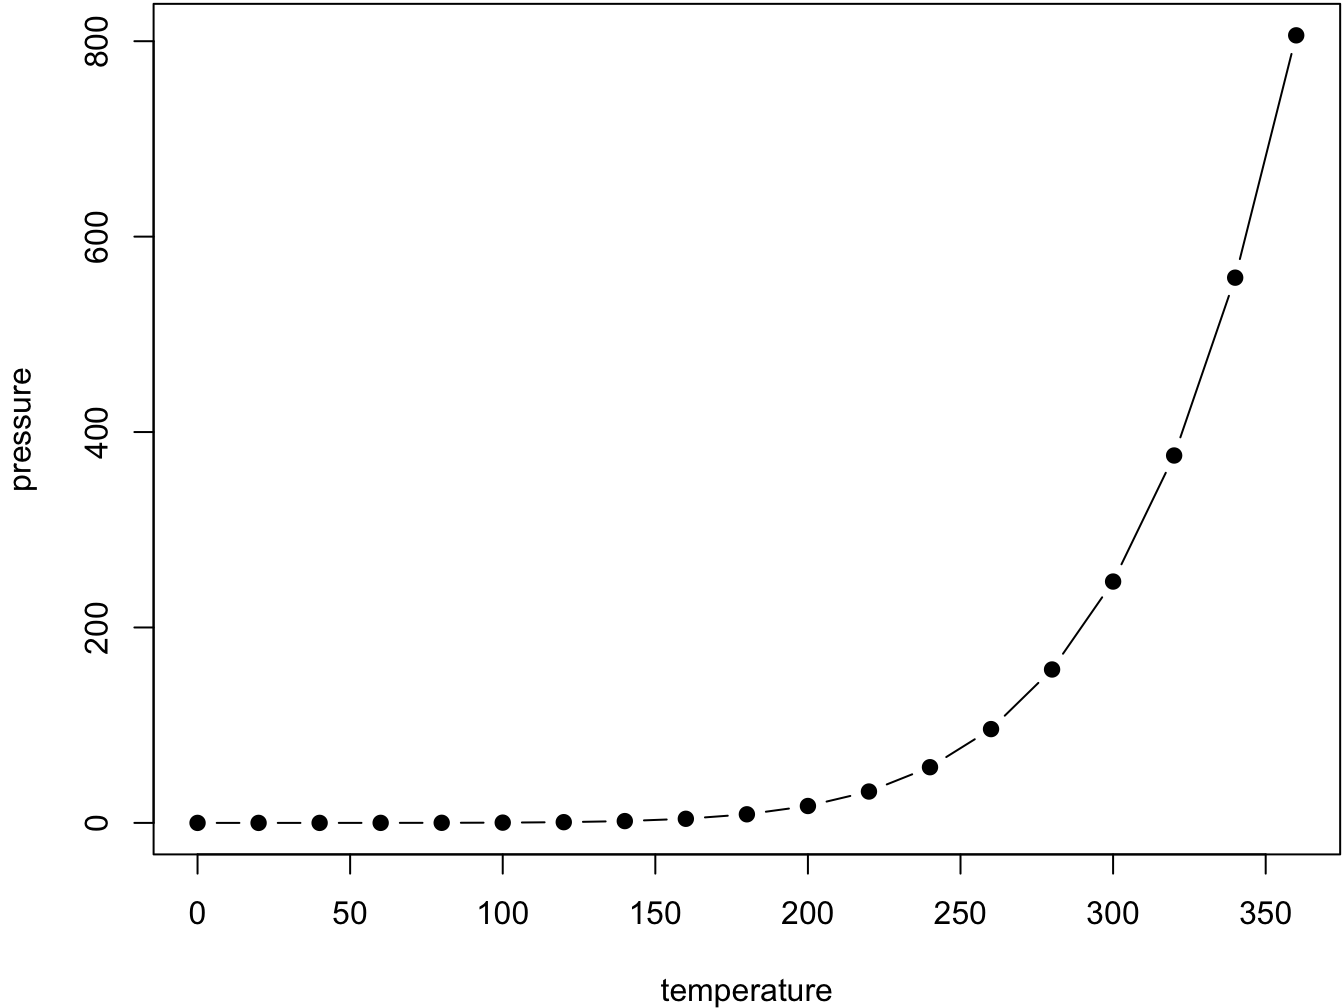
\includegraphics[width=0.8\linewidth]{QuantLife_files/figure-latex/nice-fig-1} 

}

\caption{Here is a nice figure!}\label{fig:nice-fig}
\end{figure}

Reference a figure by its code chunk label with the \texttt{fig:} prefix, e.g., see Figure \ref{fig:nice-fig}. Similarly, you can reference tables generated from \texttt{knitr::kable()}, e.g., see Table \ref{tab:nice-tab}.

\begin{Shaded}
\begin{Highlighting}[]
\NormalTok{knitr}\OperatorTok{::}\KeywordTok{kable}\NormalTok{(}
  \KeywordTok{head}\NormalTok{(iris, }\DecValTok{20}\NormalTok{), }\DataTypeTok{caption =} \StringTok{\textquotesingle{}Here is a nice table!\textquotesingle{}}\NormalTok{,}
  \DataTypeTok{booktabs =} \OtherTok{TRUE}
\NormalTok{)}
\end{Highlighting}
\end{Shaded}

\begin{table}

\caption{\label{tab:nice-tab}Here is a nice table!}
\centering
\begin{tabular}[t]{rrrrl}
\toprule
Sepal.Length & Sepal.Width & Petal.Length & Petal.Width & Species\\
\midrule
5.1 & 3.5 & 1.4 & 0.2 & setosa\\
4.9 & 3.0 & 1.4 & 0.2 & setosa\\
4.7 & 3.2 & 1.3 & 0.2 & setosa\\
4.6 & 3.1 & 1.5 & 0.2 & setosa\\
5.0 & 3.6 & 1.4 & 0.2 & setosa\\
\addlinespace
5.4 & 3.9 & 1.7 & 0.4 & setosa\\
4.6 & 3.4 & 1.4 & 0.3 & setosa\\
5.0 & 3.4 & 1.5 & 0.2 & setosa\\
4.4 & 2.9 & 1.4 & 0.2 & setosa\\
4.9 & 3.1 & 1.5 & 0.1 & setosa\\
\addlinespace
5.4 & 3.7 & 1.5 & 0.2 & setosa\\
4.8 & 3.4 & 1.6 & 0.2 & setosa\\
4.8 & 3.0 & 1.4 & 0.1 & setosa\\
4.3 & 3.0 & 1.1 & 0.1 & setosa\\
5.8 & 4.0 & 1.2 & 0.2 & setosa\\
\addlinespace
5.7 & 4.4 & 1.5 & 0.4 & setosa\\
5.4 & 3.9 & 1.3 & 0.4 & setosa\\
5.1 & 3.5 & 1.4 & 0.3 & setosa\\
5.7 & 3.8 & 1.7 & 0.3 & setosa\\
5.1 & 3.8 & 1.5 & 0.3 & setosa\\
\bottomrule
\end{tabular}
\end{table}

You can write citations, too. For example, we are using the \textbf{bookdown} package \citep{R-bookdown} in this sample book, which was built on top of R Markdown and \textbf{knitr} \citep{xie2015}.

\hypertarget{literature}{%
\chapter{Literature}\label{literature}}

Here is a review of existing methods.

\hypertarget{methods}{%
\chapter{Methods}\label{methods}}

We describe our methods in this chapter.

\hypertarget{applications}{%
\chapter{Applications}\label{applications}}

Some \emph{significant} applications are demonstrated in this chapter.

\hypertarget{example-one}{%
\section{Example one}\label{example-one}}

\hypertarget{example-two}{%
\section{Example two}\label{example-two}}

\hypertarget{final-words}{%
\chapter{Final Words}\label{final-words}}

We have finished a nice book.

  \bibliography{book.bib,packages.bib}

\end{document}
